\documentclass[authoryear,12pt, 3p]{elsarticle} 
% This version: 07FEB25-14:00 - This version was submitted to JPubE 
\usepackage{lineno}
\usepackage[utf8]{inputenc}
\usepackage[british]{babel}
\usepackage[table, usenames,dvipsnames]{xcolor}
\usepackage{enumitem}
\usepackage{amsmath}
\usepackage{amsfonts}
\usepackage{amssymb}
\usepackage{mathrsfs}
\usepackage[nice]{nicefrac}
\usepackage{xfrac}
\usepackage{subcaption}
\usepackage{ntheorem}
\usepackage{circledsteps}
\usepackage{booktabs}
\usepackage{tikz}
\usetikzlibrary{calc}
\usepackage[breaklinks]{hyperref}
\hypersetup{colorlinks, 
	urlcolor=red}
\theoremstyle{break}

\newtheorem{lem}{Lemma}
\newtheorem{thm}{Theorem}
\newdefinition{definition}{Definition}  
\newproof{pf}{Proof}
%\newproof{pot}{Proof of Lemma}

\journal{Journal of Urban Economics}

\begin{document}
	
\begin{frontmatter}
\title{Autonomy and Accountability: Strategic Behavior of German State Leaders During the COVID-19 Pandemic}
\author[1]{Salvatore Barbaro\corref{cor1}} \ead{sbarbaro@uni-mainz.de}
\author[2]{Reyn van Ewijk}
\author[3]{Julia M. Rode}

		
\affiliation[1]{organization={Johannes-Gutenberg University},
	addressline={Interdisciplinary Public Policy},
	city={Mainz},
	postcode={55129},
	state={RP},
	country={Germany}}

\affiliation[2]{organization={Johannes-Gutenberg University},
	addressline={Chair of Statistics and Econometrics},
	city={Mainz},
	postcode={55129},
	state={RP},
	country={Germany}}		

\affiliation[3]{organization = {Deutsche Bundesbank},addressline={Wilhelm-Epstein-Straße 14}, 
	city={Frankfurt}, postcode={60431}, state = {HE}, country={Germany}}

\cortext[cor1]{Corresponding author}

\begin{abstract}
The COVID-19 pandemic presented governments with unprecedented challenges, requiring decisions that balanced public health measures against substantial social and economic impacts. This study examines the strategic and opportunistic behaviors of regional officials in Germany during the pandemic. Using a comprehensive empirical analysis based on hundreds of statements from state incumbents, we shed light on the dynamics of state level political behavior.

Our findings reveal that German regional leaders emphasized their autonomy when performance metrics were favorable but strategically shifted responsibility when outcomes were less favorable. This behavior underscores the dual potential of federal systems as both laboratories of democracy and breeding grounds for responsibility-avoiding (opportunistic) behavior.
\end{abstract}
		
		%%Research highlights
\begin{highlights}
\item German state leaders emphasized autonomy when infection rates were low but shifted responsibility to the federal level when rates were high.
\item Approximately 900 public statements were analyzed to assess leaders' strategic behavior during the COVID-19 pandemic.
\item Higher state-level infection rates increased the likelihood of advocating for centralized decision-making.
\item Public statements were strategically timed around periods of heightened public attention, such as prime minister conferences.
\item The study highlights federalism's dual role as a laboratory of democracy and a platform for responsibility avoidance.
\end{highlights}
		
\begin{keyword}
Political Behavior \sep Federalism \sep Accountability \sep Yardstick competition

\JEL D72, D78,  H77
\end{keyword}
\end{frontmatter}
	
\linenumbers
%\tableofcontents
%\tableofcontents
	
\section[Introduction]{Introduction}\label{sec.introduction}
The responsibilities borne by governments during the COVID-19 pandemic were arguably the greatest in decades. Their decisions carried far-reaching consequences. The health—and lives—of thousands were at risk if governments failed to implement necessary measures to protect against the virus. Conversely, restrictions on assembly and freedom of movement had severe repercussions, like  economic hardship and children unable to attend school. Each decision risked triggering social and economic disruptions, and clear `right' or `wrong' answers to critical questions were often absent.

In such circumstances, government's ability to learn from one another becomes crucial. Federal systems are often seen as particularly strong in this regard. Regional governments make decisions that may perform better or worse, enabling others to learn and adapt, fostering a competition of ideas within the federal framework. Justice D. Brandeis famously described states as \textit{laboratories} of democracy, conducting political experiments\footnote{Brandeis noted in 1932 in the New State Ice Co v. Liebman case (285 US. 262, 311) that ``a single courageous State may serve as a laboratory; and try novel social and economic experiments without risk to the rest of the country.''}.

Whether this vision of federalism holds true or remains a romanticized `campfire tale' \citep{Tyler2022} is debated. Critics question whether political competition truly fosters independent decision-making, policy innovation, and progress \citep{RoseAckerman1980, Weaver1986, Strumpf2002}. While competition may encourage bold experimentation, it is risky for weak or low-performing state incumbents. However, other scholars take a more optimistic view, arguing that federal competition can be a driver of innovation. They suggest that state politicians, particularly those with aspirations at the federal level, have strong incentives to implement successful policies, as doing so enhances voters' perceptions of their competence \citep{KotSchwager2006}.

James Madison grappled with these questions, asserting that federal systems succeed when both central and state governments accept divided authority and exercise independent power. However, opportunistic behavior poses a significant challenge, as Madison noted in his \textit{Vices of the Political System of the United States} \citep{Madison1787}. Depending on whether outcomes are favorable or adverse, the leaders of regional governments can utilize the federal structure to either claim responsibility or to avoid being perceived as decision-makers and instead attribute responsibility to the federal level.

Whether federal systems are used by regional politicians as convenient features that allow them to claim or shift away responsibility opportunistically, is challenging to investigate \citep{Agrawal2022}. For example, one needs to be able to observe how the same or similar politicians behave when outcomes in their polity are more vs less favorable. This, moreover, requires more or less objective measures of policy success that are at the same time very salient to the general public. Moreover, there should be some degree of randomness in terms of these outcomes. 

The COVID-19 pandemic provides a unique opportunity to examine state incumbents' strategic and opportunistic behavior. The global shock captured extraordinary public interest, ensured comparable challenges across regions, and, in Germany--the country we study, highlighted the tension between autonomous state decision-making and federal oversight.

While voter interest in policy decisions was high, at the same time, statistics on regional incidence rates were readily available in Germany and were closely watched by the general public. This made governments highly accountable \citep{Neundorf2021, Algara2022, Singer2022, Kennedy2022}. If incidence rates in one state increased considerably compared to the average of all other states, then the public would be inclined to regard this as a poor performance of the regional government’s handling of the pandemic. Conveniently for our setup, it was, however, often unclear whether changes in incidence rates were due to these regional governments or not. This is firstly because the pandemic was a worldwide shock that afflicted German regions in a comparable fashion. Some regions may overall have been impacted more than others, e.g., due to their greater reliance on manufacturing, but this can be controlled for. Once one does so, most states have seen periods during which infection rates were higher or lower than expected. Secondly, both the federal and the state governments were responsible for managing the pandemic response. However, the distribution of competences between the federal tiers was not clearly assigned. In Germany, the task of public health protection is primarily a matter for the states, yet the federal government was able to broadly assert jurisdiction through concurrent legislation (see Subsec. \ref{FederalStructure}). The states could make significant decisions, such as school closures, entirely autonomously or refer to nationwide agreements. This particular institutional environment enables an investigation on whether regional politicians either claim or shift responsibility. 

In order to link whether politicians take credit or shift blame in response to favorable or unfavorable outcomes, we use approximately 900 official statements made by prime ministers of German federal states. These were mainly made via Twitter, and we classified these via a standardized coding scheme.

Our empirical assessment suggests that leaders emphasized independent decision-making when performance metrics were favorable but avoided responsibility when outcomes were less advantageous. This effect is even more pronounced when we focus on time windows in which public statements attracted particularly high attention.

Thus, we find empirical support for James Madison’s concern that federal systems may fail to realize their potential strength due to strategic or opportunistic considerations by leaders in the constituent units. This, in turn, undermines the appeal of federalism as \textit{laboratories}.


\section[Federalism in Germany]{Institutional Background: Federalism in Germany}\label{FederalisminGermany}
%
\subsection[The federal structure]{The federal structure}\label{FederalStructure}
Germany's constitution does not prescribe federalism in a refined form, nor does it establish a powerful central government. The term 'unitary federal state' \citep{Hesse1962, Turner2013} aptly characterizes this blended status.\footnote{
	Article 30 of the Basic Law presumes that governmental powers lie with the Länder unless the Basic Law provides otherwise, akin to the Tenth Amendment of the U.S. Constitution. In practice, however, Article 30 was rarely enforced and was labeled a 'living lie' by \cite{Scharpf1994}. Furthermore, Article 70 qualifies Article 30 by stating that the Länder have the right to pass legislation only to the extent that the Basic Law does not grant authority to the central tier.
} The federal polity is often regarded as the archetype of administrative federalism and cooperative decision-making \citep{Kropp2016}. On the federal level, the Länder are represented in the second parliamentary chamber (Bundesrat). They hold a vote on federal laws that trigger the establishment of new administrative proceedings or agencies on the state level \citep{Burkhart2008}, or that impact states' revenues. 

A particular feature in Germany's constitutional framework are concurrent legislation \citep{Gunlicks2007}, which applies to a variety of policy fields. Among them is the public health responsibility. Concurrent legislation denotes that the Länder maintain legislation as long as the federal tier makes no use of its legislative powers in the same field. In this respect, concurrent legislation offers both sides, the states as well as the federal government, opportunities for abdication.

\subsection{Public health responsibilities in Germany's federal polity}
The legal framework governing government intervention during a pandemic is established by the Infection Protection Act (Infektionsschutzgesetz, IfSG). The Länder administer this law, exercising discretion in determining specific measures, their severity, timing, and scope. While the IfSG empowers the federal government to issue recommendations, it also promotes coordination among federal states while allowing flexibility for their actions \citep{Tonti2022}.  

State governments have enacted several measures to curb infections, like the imposition of curfews and limitations on the assembly right, the closing of educational institutions, restaurants, stores, and other facilities. The federal government has retained jurisdiction over border controls. Extensive financial aid packages have been designed by the federal, but were co-financed by the states.\footnote{ 
	The legal framework in Germany also allowed municipalities to chart their own course. Some cities began to take advantage of this opportunity early in the pandemic. The most prominent example is Jena, which was the first city to introduce a requirement for wearing face masks very early on. It became evident that the city of Jena thus generated a prime example of a political laboratory. \cite{Mitze2020} showed that the city’s introduction of masking requirements led to an approximate 25\% reduction in the infection numbers three weeks following introduction. The success in Jena fostered the nationwide compulsory masking.
} 

As mentioned in the previous subsection, the federal government had the option to take over the tasks handled by the states. However, the federal government did not exercise this authority for the longest time, but only in the summer of 2021 \citep{Rowe2023}, when the pandemic had relaxed and most restrictions were lifted.

\subsection{Response to the COVID-19 pandemic in Germany's federalism}
Germany was able to weather the COVID-19 pandemic relatively well compared to other industrialized nations. Infection rates, particularly in the autumn of 2020, were relatively low, thus avoiding widespread strain on the healthcare system. 
\begin{figure}[h]
	\centering
	\includegraphics[width = \linewidth]{berfig01.pdf}
	\caption{COVID-19 infections in Germany compared to the other G7 countries and among German states. Source: \cite{Guidotti2022}}
	\label{fig.sevendayincidence}
\end{figure}
The public paid particular attention to infection rates, which were reported by the national health authority in the form of a seven-day incidence rate. This rate is calculated as a moving average over seven days and is expressed in relation to 100,000 inhabitants. The left panel in Fig. \ref{fig.sevendayincidence} depicts this indicator in Germany and the other six G7 countries.

Although infection rates on average were moderate, there were significant differences within Germany (i.e., between the federal states). The right panel in Fig. \ref{fig.sevendayincidence} illustrates the infection rates of the sixteen Länder and marks the nationwide average by the orange-colored line. The public closely monitored these values because they were ultimately viewed as the central measure for the possibility of easing the imposed restrictions. Thus, citizens carefully compared how the numbers in their federal state developed compared to other federal states and to the national average \citep{Kaatz2022}.

The national infection control agency, the Robert Koch Institute, which collected and published data on the pandemic, categorizes the infection dynamics into three waves, which are graphically depicted in the right display of Fig. \ref{fig.sevendayincidence}. Wave 1 ran from February 2nd, 2020 till May 17th, 2020; wave 2 from September 28, 2020 till February 28th, 2021, and wave 3 from March 1st, 2021 till June 13th, 2021.

\begin{figure}[h]
	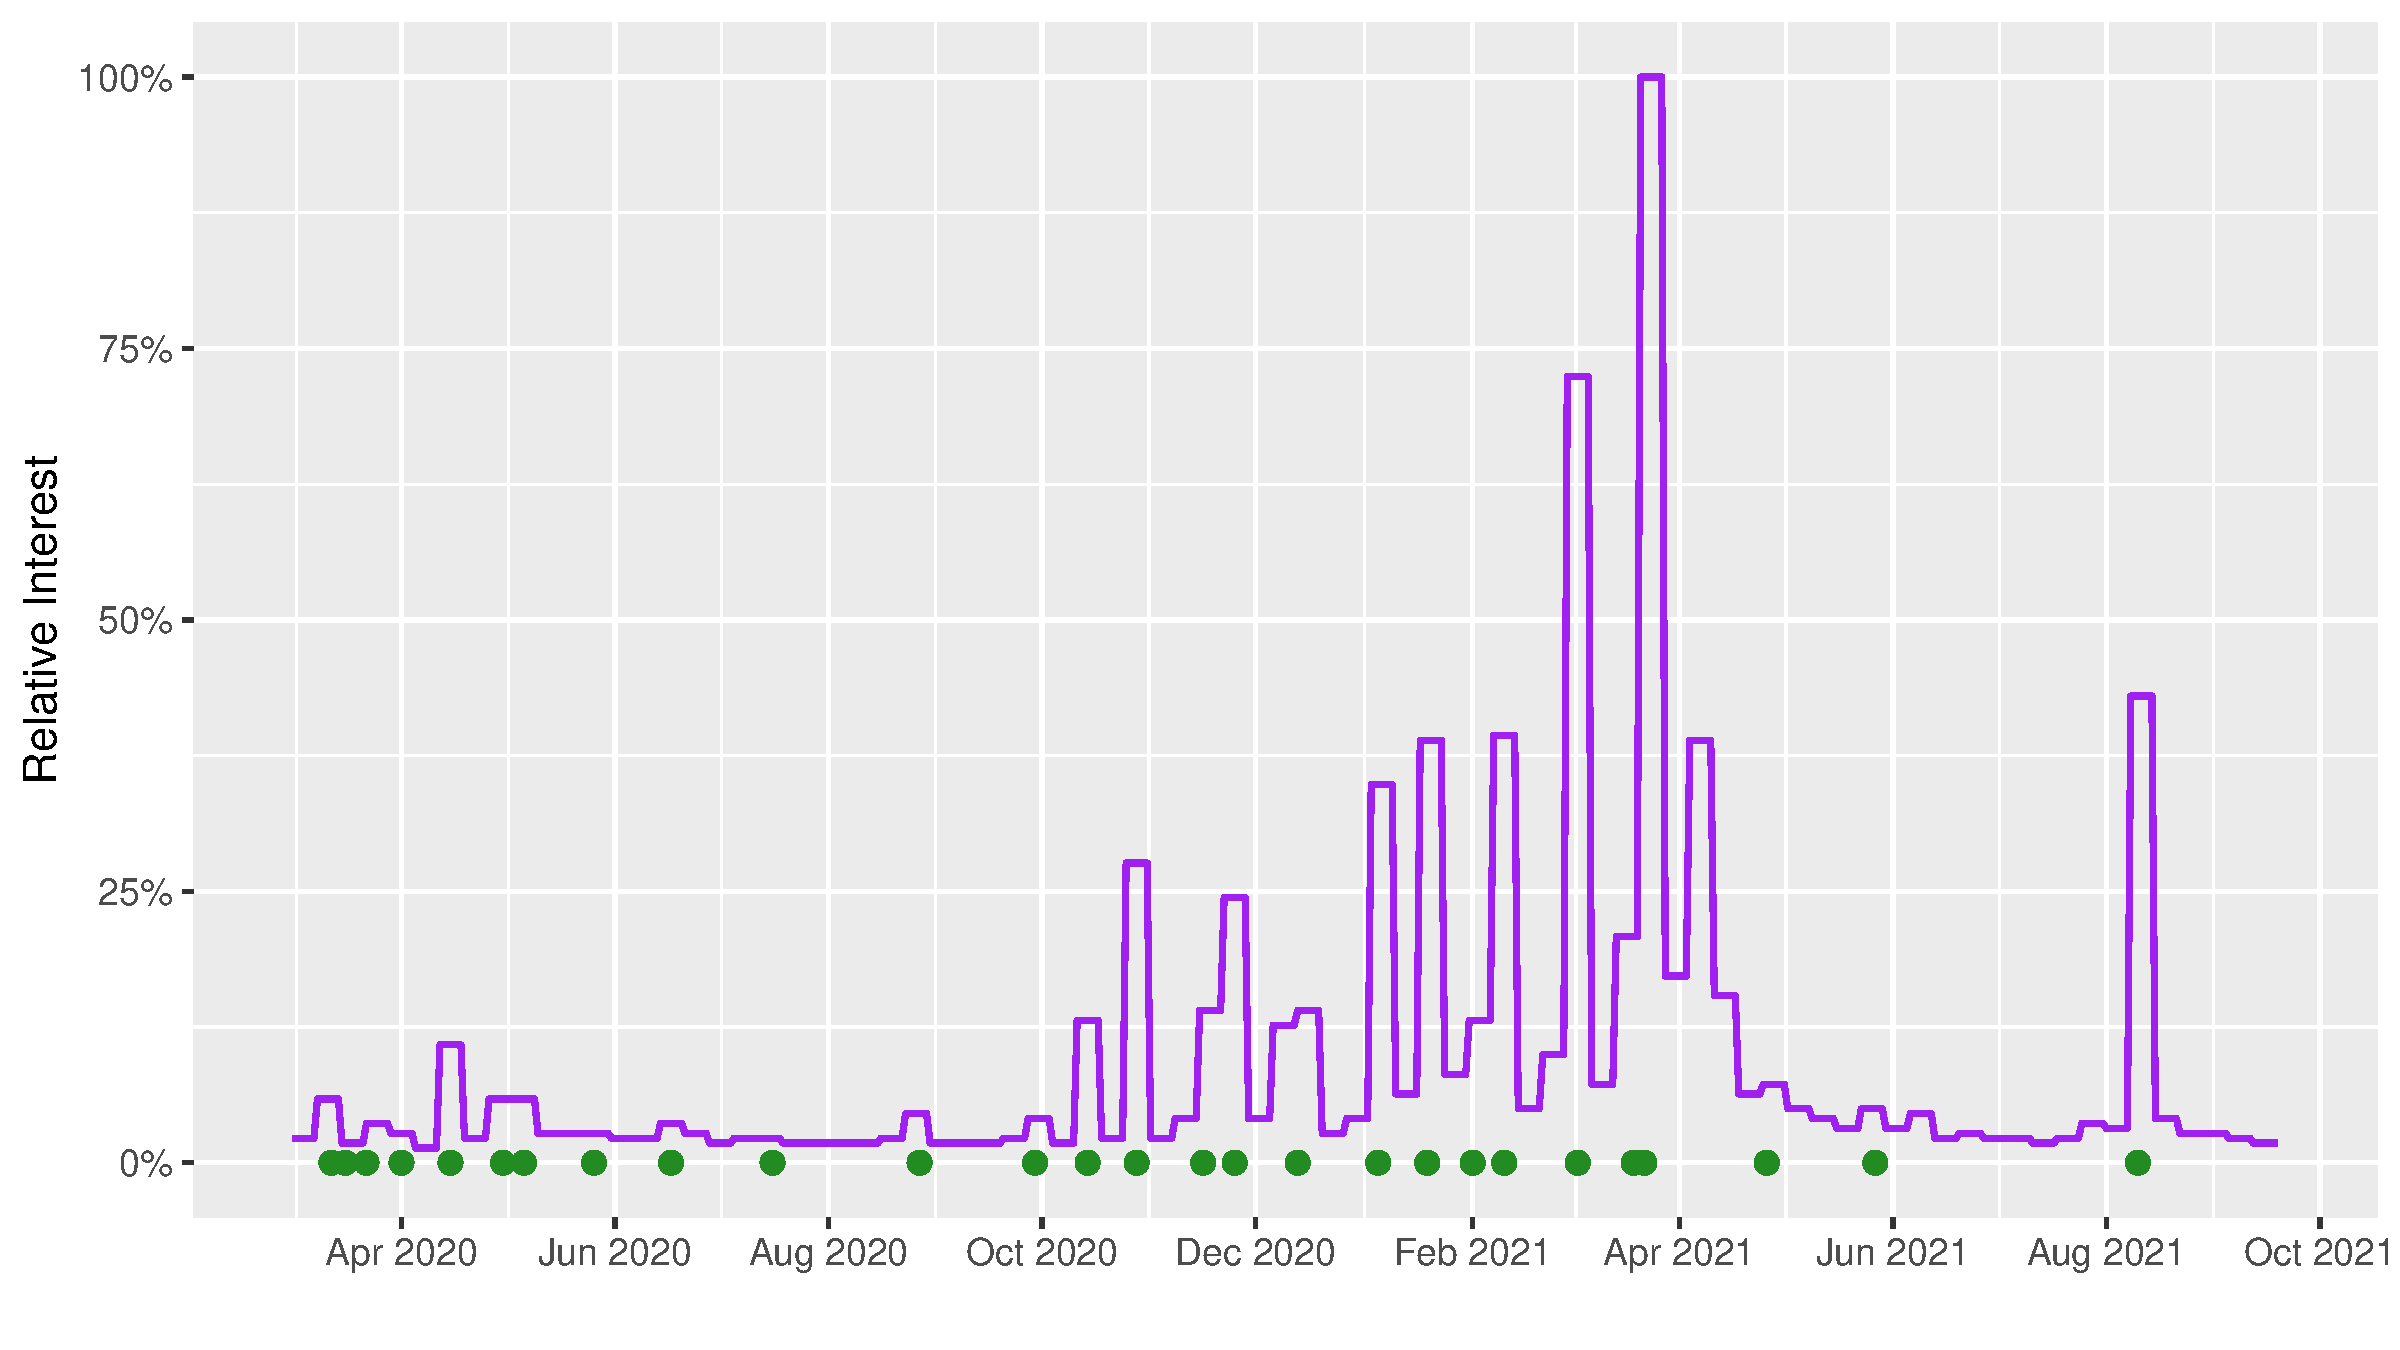
\includegraphics[width=\linewidth]{mpk2}
	\caption{Google hits for joint conferences (and related search items).}
	\label{fig.mpk}
\end{figure}

Shortly after the pandemic's onset, state governments were highly interested in policy coordination in joint meetings of states' prime ministers with the chancellor. During the joint meetings, which initially took place quite frequently, the heads of governments agreed on guidelines for crisis management. During the first wave, coordination and uni-directional measures dominated policymaking. While policy decisions were homogeneous in the first months after the pandemic's onset, decisions became more heterogeneous during the second and third wave \citep{Hegele2021, Kuhlmann2021}.

In the context of this assessment, it is crucial to note the high level of public awareness regarding the outcomes of the joint meetings. To illustrate this awareness, we analyzed data from Google. Figure \ref{fig.mpk} depicts the number of Google searches for the term 'Ministerpräsidentenkonferenz' (the German term for the joint conference) and closely related terms suggested by Google (such as 'results of the joint conference'). The numbers are presented relative to the peak search volume, where a value of 60\% signifies that the searches on a given date amounted to 60\% of the searches on the day with the highest volume. The green dots mark the dates on which the joint conferences occurred. Figure \ref{fig.mpk} indicates that the public showed significant interest in the outcomes of these joint conferences.

Not only did public attention increase rapidly around the time of the meetings, but the statements and opinions of the prime ministers also concentrated heavily on the days immediately following the conferences. We show this analytically in Section \ref{sec.results} (see Table \ref{tb.pmc}). We interpret this as an additional indicator that the conferences received high attention both from political leaders and the public.

From the second wave onwards, the conferences took place generally every third week. Despite this high frequency of coordination meetings, some states preferred to take their own measures and deviated from the measures discussed at the conference.

\begin{figure}[h]
	\centering
	\includegraphics[width=\linewidth]{lockdown2}
	%	\includegraphics[width = \linewidth]{lockdownfig.pdf}
	\caption{Stringency index for relevant restriction measures. Data source: \cite{Steinmetz2022}.}
	\label{fig.lockdown}
\end{figure}

The times and intensity of measures implemented by the Länder to contain the pandemic are summarized in a comprehensive dataset by \cite{Steinmetz2022}. Three particularly salient measures were the stay-at-home requirement ('leavehome'), the closure of schools ('school'), and the closure of childcare facilities ('daycare'). The decisions of the countries to tighten their measures in these areas or to relax the respective restrictions are illustrated in Figure \ref{fig.lockdown}.

Each vertical line denotes a measure adopted by the respective state government, either towards a more stringent regulation (value of 1 or 2) or towards a relaxation (value of 0). Each state is marked by its own color. Figure \ref{fig.lockdown} shows that during the second and especially the third wave, the states did not make their decisions synchronously. In particular, they relaxed measures earlier or later than discussed between the federal government and the states. The data also depicts the homogeneity of policy decisions during the first wave. 

\section{Data \& Methods}\label{sec.datamethods}
Our main source of data consists of statements and declarations made by prime ministers of German federal states with respect to COVID-19 management via Twitter. We obtained these data through the Twitter API \citep{Kearney2019}.\footnote{
	We filtered out tweets related to COVID-19 on the accounts of the prime ministers or their press offices.
} Additionally, we have taken into account press releases and official statements by the respective prime ministers, further enriching our analysis.\footnote{
	Prime Minister Günther of Schleswig-Holstein gave the last COVID-19 related government declaration in January 2021 and replaces them afterwards with oral reports. From Jan. 20th, 2021, these COVID-19-related oral reports are included instead of government declarations. Prime Minister Laschet of North Rhine-Westphalia does not give government declarations during the time of interest. Instead, we utilize COVID-19-related briefings of this state’s government to its local parliament.}

Statements are considered if they indicate preferences/information about the stance of the prime minister regarding centralized or decentralized decision-making. We construct an index measuring state governments’ positioning during the COVID-19 pandemic. This ``pandemic policy index" (\textbf{PPI}) measures the extent to which a prime minister, at a given moment during the COVID-19 pandemic, attempts to shift responsibilities to the federal government, the second parliamentary chamber and/or the prime minister conferences. On the one extreme, a Prime Minister can insist on nationwide regulations or criticize the federal government for not implementing uniform nationwide rules. At the other extreme, a prime minister can state that his/her state will act alone or criticize that the federal government encroaches too much.

Each statement is categorized into four distinct and mutually exclusive categories using an ordinal scale. A value of one indicates that a state prefers to act individually, while a value of four indicates that it asks for more action on the federal level or blames it for problems. Making statements belonging to categories one and two can be interpreted as expressing a preference for federalistic decision-making, and conversely, making statements belonging to categories three and four can be interpreted as expressing a preference for unitary decision-making.

We have summarized our criteria for categorizing all statements in \ref{app.category}. We also provide in this Appendix two translated examples to illustrate how we applied the categories to the statements.

Categorization criteria were thoroughly predefined in order to ensure a high reliability of the scale. The interrater reliability was tested by rating the same statements three times independently. The coders had been trained in the use of the \textbf{PPI} rates. The interrater-reliability was calculated using Fleiss’ $\kappa$ \citep[][Ch.~18]{Fleiss2003}, which is a generalization of Cohen’s kappa for cases with more than two raters. The $\kappa$ statistic compares the observed level of agreement between coders (judges, observers) to the level that is expected under chance. If there is no agreement among coders, then ${\kappa}$ hovers around zero, while ${\kappa}=1$ indicates perfect agreement. Following \cite{Fleiss2003}, a $\kappa$-statistic greater than 0.75 indicates an ``excellent'' level of agreement. In our case, $\kappa$ was 0.91, which implies that rating using the \textbf{PPI} was done reliably and consistently.

Our dataset relies on 600 prime minister statements. Of these, 35.5\%, 6.2\%, 44.8\% and 13.5\% were classified with index values 1, 2, 3 and 4, respectively.

In our study, we investigate whether state governments adapt their stances opportunistically based on their own performance. Specifically, we examine if they favor decentralized decision-making when their performance is good, and shift towards centralized decision-making when their performance is poor. 

The lower the state-level rate compared to the national average, the better the state's performance. An advantage of this measure is that the data were collected by an authoritative national agency and were widely regarded by the population.

The main ordered logistic regression equation for our analyses is:
\begin{equation} \label{eq.regression01}
	\ln \left( \frac{P(Y \leq j)}{P(Y > j)} \right) = \beta_{j0} + \beta_1 \ln(\text{\texttt{incstate}}_{it}) + \beta_2 \ln(\text{\texttt{incfed}}_{t}) + X' \gamma + u_{it} 
\end{equation}
in which $\frac{P(Y \leq j)}{P(Y > j)}$ is the odds of giving a statement falling into category $j$ or lower. $\beta_{j0}$ for $j \in \{1,\ldots,4\}$ give the four category-specific intercepts. \texttt{incstate}$_{it}$ is the incidence rate for state $i$ on date $t$, and \texttt{incfed}$_{t}$ is the federal-level incidence rate on date $t$. In our results, we report the exponent of each coefficient ($\mathrm{e}^{\beta_1}$, etc.) so that the interpretation is in odds. Coefficients larger than 1 imply that an increase in a variable leads to an increase in the odds of giving a statement that lies in a higher category. 

We take the natural logarithm of both \texttt{incstate}$_{it}$ and \texttt{incfed}$_{t}$, so that the coefficient $\mathrm{e}^{\beta_1}$ gives the increase in the odds of giving a higher category statement when the ratio of incidence rate at the state-level divided by incidence rate at the federal level doubles.

An alternative would have been not to include both these variables, but instead measure the deviation between state and federal incidence rate as  $\frac{\text{\texttt{incstate}}_{it} - \text{\texttt{incfed}}_{t}}{\text{\texttt{incfed}}_{t}}$, for which for example a value of zero means that the state rate equals the federal one, and a value of one indicates that the state rate is double that of the federal one. Both specifications only differ in their functional form assumptions. We will show a robustness check in which we demonstrate that the estimated effect sizes in both cases are virtually identical.

In our regression equation, the matrix $X$ includes a set of covariates. These will be included in our regressions in several steps. First, we will control for a linear time trend to capture a potential general trend in stances regarding federalistic decision-making. Next, we include a dummy for the five East German states, and a dummy for the state of Berlin, as there may be differences in policies and attitudes between these states and the western ones. 

Next, we control for a set of state-level variables. First among these is the fundamental stance of the state government towards federalism. If a state advocates increased de/centralization, this will not necessarily be driven solely by opportunistic or strategic considerations; ideological convictions can often supersede pragmatic political interests. For example, in the USA, it is known that ideological convictions play a pivotal role in shaping states' and citizens' preferences toward de/centralization. Specifically, conservatives exhibit a genuine attachment to decentralization, while attitudes toward federalism tend to be more instrumental among liberals \citep{Glaser2023, Rendleman2022}. In our context, take, for example, a state government with above-average incidence rates that advocates for decisions regarding school closures or openings to be made collectively and implemented uniformly across the federation. This stance may be opportunistic if the state government generally favors decentral (i.e., federalistic) decision-making. Still, it may also be congruent with a fundamental belief that the respective state harbors no sympathy for the autonomy of states.

For the variable measuring the fundamental stances of state governments towards federalism, we used data from \cite{BarbaroRode2024}, who determined these general stances based on each state's coalition agreements prior to the outbreak of the COVID-19 pandemic. The data were classified such that a designation of one signifies a promotion of strong federalism, while four indicates a willingness to cede competencies to the federal level. Each state's resulting average attitude-index values toward federalism are visualized in \ref{app.stances}, Figure \ref{fig.attitudemap}. 

In this step, we furthermore control for states’ pre-pandemic (2019) share of the manufacturing sector in their gross value added. This variable shows how severely the COVID-19 pandemic affected each state's economy \citep{Flach2020}. Furthermore, we control for states’ financial strength, measured as the sum of states’ tax revenues and the tax revenues of their municipalities, which, in Germany, is referred to as states’ financial capacity (“Finanzkraftmesszahl”). 

In the German redistributive system, financially weak states receive funds out of other states' financial means and additional federal government grants (“financial equalization”). This may affect their stances toward federalistic vs decentral decision-making.\footnote{
	We use 2021 data for this as data for this year most accurately reflect the situation during the pandemic. Moreover, data for pre-pandemic years are less useful as the financial equalization scheme has been reformed. The German statistical office (Statistisches Bundesamt) provides data for this measure.
}  

In the final step, we control for the natural logarithm of the state and federal vaccination rates at each given date. Data on state- and national-level vaccination rates are available from the epidemiological database for COVID-19 \citep{Guidotti2022}. 

Both variables receive the value $0$ for dates before vaccinations started, and a dummy variable for the pre-vaccination period is included. State vaccination rates, relative to federal vaccination rates, can be thought of as another measure of the success of local policies, although they less clearly result from policies and interventions at the state level than from incidence rates.\footnote{
	The federal government procured the vaccine doses, but the states organized the vaccinations. Each state had its own vaccination centers and procedures for scheduling vaccination appointments. For example, some states offered vaccinations on buses that traveled to university campuses and smaller towns. Therefore, high vaccination rates can be attributed to the respective states' high administrative quality.
} Moreover, access to vaccinations was only possible starting in January 2021.  

Our analyses utilize prime minister statements from waves 2 and 3 of the pandemic. Before wave 2 started, incidence rates were considerably less reliably recorded. Measurement error in the initial phase of the pandemic may have differed between states and potentially so in an endogenous way. Moreover, during wave 1, and especially the period between waves 1 and 2, the difference between state-level and federal-level incidence rates measured in percentages fluctuated wildly as reported rates were often low.

In our ordered logistic regression, the coefficients $\beta_1$, $\beta_2$, and $\gamma$ are assumed to be the same across all categories. We test this proportional odds assumption for our main model (5) using a Brant test \citep{Brant1990} and find no evidence for a violation of this assumption: the null hypothesis of equality of the coefficients is not rejected with $\chi^2 (22) = 28.7$, $p = 0.154$. 

Standard errors are clustered at the date level to account for any between-state correlations that arise because during the pandemic all states often experienced similar events (e.g., pandemic-related news) at the same moment.  

During our study period, the prime ministers of North Rhine-Westphalia and Bavaria fiercely and publicly contested the chancellor candidacy of the conservative parties (CDU and CSU). Both tried to distinguish themselves with their own positions on handling the pandemic \citep{Jun2023}. Therefore, it is possible that the internal party campaign biased the statements of these two prime ministers. We excluded these two states in a robustness check to account for this.

In a further robustness check, we conduct a state fixed effects (conditional) ordered logistic regression. This has the advantage of relying solely on within-state variation but has two drawbacks. First, we lose a lot of the variation of interest and, therefore, statistical power. Second, this method cannot be estimated when the clustering of the standard errors is at a different level (here: date) than the grouping variable (here: state). Hence, some relevant autocorrelation is ignored, while clustering occurs for a low number of groups (16 states), which might lead to inconsistent standard errors.

During the pandemic, the joint conferences of the state prime ministers were closely watched by the population as many of the central pandemic-related interventions were discussed and decided upon. We expect that prime ministers will have been especially likely to make their stance with respect to centralized or decentralized decision-making clear in the week around these conferences, and perhaps most so in the days immediately following such a conference. We, therefore, conduct two sets of analyses. First, we analyze to what extent the number of statements issued per day changed during the week of a conference (three days before, three days after the conference) and immediately subsequent to a conference (day of the conference till three days afterward). For this, we calculate the number of statements issued daily and regress this on a linear time trend with a dummy indicating the time period right around / right after the prime ministers' conference. Second, we conduct our main analyses using the specification that includes all controls while limiting the data to the time period right around / right after prime ministers' conferences.

\section{Results}\label{sec.results}
\subsection{Main Analysis}

The results of the regression analyses using Equation (\ref{eq.regression01}) are shown in Table \ref{tb.reg01}, with the last three rows representing the covariates. The dependent variable is a 4-point ordinal scale with higher scores indicating a stronger preference for unitary (centralized) decision-making.

\begin{table}[htbp] 
	\centering
\caption{Covid-19 incidence rates and state prime ministers' statements favoring (de)centralized decision-making}
 \label{tb.mainreg}
\begin{tabular}{lccccc} \toprule
    & (1) & (2) & (3) & (4) & (5) \\ \midrule
ln(state-level  & 1.730** & 1.904*** & 2.003*** & 1.983** & 1.985** \\
\, incidence rate)	& [1.22,2.45] & [1.34,2.70]  & [1.41,2.85]  & [1.30,3.02]  & [1.29,3.06] \\
 & & & & & \\
ln(state-level  &  &  &  &  & 0.806 \\
\, vacc. rate)		&  &  &  &  & [0.606,1.072] \\
		& & & & & \\
Linear time trend & No & Yes & Yes & Yes & Yes \\
		& & & & & \\
Dummies Eastern  &    &    &     &     & \\
\,  states and Berlin  & No & No & Yes & Yes & Yes \\ 
		& & & & & \\
State-level controls & No & No & No & Yes & Yes \\ \\ \midrule
 Observations & 600 & 600 & 600 & 600 & 600 \\		\bottomrule
\end{tabular}
\label{tb.reg01}
\begin{minipage}{\textwidth}
	\small
\textit{Notes:} Each column reports exponentiated coefficients from a separate ordered logit regression. Dependent variable is the 4-point pandemic policy index (PPI). Higher values indicate a stronger expressed desire for centralized decision-making. Coefficients are expressed as changes in the odds ratio of giving a statement $Y$ that falls into a higher vs a lower category $j$, i.e., $P(Y\leq j)/P(Y > j)$. All regressions control for ln(federal level incidence rate) and column (5) additionally controls for ln(federal level vaccination rate) and a dummy for the pre-vaccination period. State-level controls include states' general stances towards federalism, share of the manufacturing sector in gross value added, and financial strength ("Finanzkraftmesszahl"). \newline \textit{*** $p < 0.01$, ** $p < 0.05$, * $p < 0.10$}
	\end{minipage}
\end{table}

The table presents exponentiated coefficients from an ordered logistic regression. The coefficients to the natural log of state-level incidence rates give the increase in odds $\left( \frac{P(Y \leq j)}{P(Y > j)} \right)$ of giving a statement that falls into category $j$ or lower. Coefficients larger than one indicate that an increase in an independent variable leads to higher scores on the \textbf{PPI}, while coefficients smaller than one indicate the opposite. Increases in incidence rates in a state relative to the country-wide level lead prime ministers to display a greater preference for centralized decision-making. If the incidence rate in a state doubles compared to that at the federal level, the odds of giving a statement that is categorized as being one point higher on the \textbf{PPI} also roughly doubles.

As can be seen by comparing columns (1) to (5), the main result is robust throughout all specifications. The coefficient to the log of the state-level vaccination rate suggests that higher vaccination rates in a state, compared to the nationwide average, lead prime ministers to give statements that are more federalistic in nature, i.e., more strongly in favor of decentralized decision-making. However, this estimate does not reach significance at conventional levels.

In \ref{app.fullregtab}, we will present models (4) and (5) in an extended form, with the specific coefficients of the covariates listed individually. As can be seen from this more comprehensive table, the coefficients to none of the three variables reach significance. The coefficient to the variable measuring states’ general stances towards federalism suggests that states that had been strongly in favor of centralization before the pandemic became relatively less so during the pandemic, and vice versa.

\subsection{Robustness Checks}
As outlined in the previous section, we conducted a series of robustness checks. The first concerns the two prime ministers who were in an intra-party competition during the observation period. In fact, these two prime ministers made the highest number of statements. Therefore, this intra-party campaign could distort the results. As part of our first robustness check, we repeated the regression analysis from  Table \ref{tb.reg01}, column (5), but without the data from these two states, which results in the loss of 121 observations.

\begin{table}[htbp]
%	\centering
\caption{Robustness checks: COVID-19 incidence rates and state prime ministers' statements favoring (de)centralized decision-making}
\begin{tabular}{lcccc}		\toprule
  & Excluding NW & Deviations in- & Fixed & Fixed \\
  & and BY       & stead of logs & effects & effects \\
  & (1) & (2) & (3) & (4) \\	\midrule
ln(state-level  & 2.145*** &  & 1.610 & 1.504  \\
\, incidence rate)  & [1.38,3.33] &  & [0.91,2.86] & [0.86,2.63]   \\
  & & & & 			\\
ln(state-level   & 0.751* &  & & 0.740**   \\
\, vacc. rate)  &   [0.58,0.97] & & & [0.56,0.98]   \\
  & & & &		\\
Perc. diff.: state- vs   &  & 1.956** &  &  \\
\, fed.-level incid. rate &  & [1.17,3.25] &  &  \\
  & & & &			\\
Perc. diff.: state- vs       &  & 0.961 &  &  \\
\, fed.-level vacc. rate	&  & [0.10,9.22]  &  &  \\
 & & & &		\\
Linear time trend & Yes & Yes & Yes & Yes \\
& & & & \\
Dummies for Eastern  & Yes & Yes & No & No \\
\, states and Berlin & & & & \\
 & & & & \\
State-level controls & Yes & Yes & No & No \\
 & & & & \\
State fixed effects & No & No & Yes & Yes \\
 & & & &		\\ \midrule
 Observations & 479 & 600 & 600 & 600 \\		\bottomrule
\end{tabular}		
\label{tb.reg02}
\begin{minipage}{\textwidth}
\small 	\textit{Notes:} Columns (1), (3) and (4) each report exponentiated coefficients from a separate ordered logit regression. In columns (3) and (4), these are state fixed effects (conditional) ordered logistic regressions. Dependent variable is the 4-point pandemic policy index (PPI). Higher values indicate a stronger expressed desire for centralized decision-making. Coefficients are expressed as changes in the odds ratio of giving a statement $Y$ that falls into a higher vs a lower category $j$, i.e., $P(Y \leq j)/P(Y > j)$. Column (2) shows results from a regression in which the independent variable of interest is measured as percent difference between state-level and federal-level rates. Regressions (1), (3) and (4) control for ln(federal level incidence rate). Regressions (1) and (4) additionally control for ln(federal level vaccination rate). Regressions (1), (2) and (4) include a dummy for the pre-vaccination period. State-level controls include states' general stances towards federalism, share of the manufacturing sector in gross value added, and financial strength ("Finanzkraftmesszahl").
\newline \textit{*** $p < 0.01$, ** $p < 0.05$, * $p < 0.10$}
\end{minipage}
\end{table}

Table \ref{tb.reg02} presents the regression results. A comparison of Tables \ref{tb.reg01} and \ref{tb.reg02} shows that the estimated effect of incidence rates on prime ministers’ stances regarding (de)centralized decision-making remains robust when the states of North Rhine-Westphalia (NW) and Bavaria (BY) are omitted from the data.

In the next robustness check, we do not include the logs of the state- and federal-level rates, but instead take the relative difference between both rates, with e.g., a value of one indicating that the state rate is double that of the federal one. The estimates are almost the same as in the main analyses.  

Finally, in columns (3) and (4), we show the results from fixed effects (conditional) ordered logistic regressions. The results should be treated with some caution because, as we pointed out at the end of Section \ref{sec.datamethods}, not all autocorrelation is taken into account, and standard errors may be inconsistent. The point estimates are robust to the inclusion of fixed effects, though coefficients are slightly smaller than in our main analyses.

Regarding the influence of vaccination rates, the robustness checks show a similar coefficient to the main analysis. However, the vaccination rate coefficient becomes significant at the 95\% level when the states of Bavaria and North Rhine-Westphalia are excluded as well as in the fixed-effects specification. The coefficients are smaller than one, which indicates that if state-level vaccination rates increase relative to the federal level, prime ministers tend to propagate more decentralized decision-making.

The significant effect of the vaccination rate coefficient may be seen as further support for our main hypothesis, according to which above-average success (in this case: higher vaccination rates than the national average) motivates the state prime ministers to emphasize the states' own responsibility and self-determination more strongly. 	

\subsection{Focusing on the time around prime ministers conferences}
The previous analyses cover all dates during the second and third waves of the pandemic. We argued that public awareness was exceptionally high on the days around the prime ministers' conferences (see Fig. \ref{fig.mpk}). This means, conversely, that statements by the prime ministers on days with lower attention are weighted the same as statements on days with very high attention to the topic of COVID-19. Prima facie, it cannot be ruled out that prime ministers will have timed those statements that were meant to most clearly convey a message right around conferences, as they knew that statements at these moments would have reached the most attention and the largest possible audiences.

\begin{table}[htbp]
%	\centering
\caption{Numbers of statements per day around prime ministers conferences (PMC)}
\begin{tabular}{lccc}	\toprule
    & (1) & (2) & (3) \\	\midrule
Week of PMC & 1.786*** &  &  \\
    & (0.492) &  &  \\
    & & &			\\
3 days before PMC &  & 0.081 &  \\
    &  & (0.422) &  \\
    & & &			\\
Day of PMC till 3 days afterwards &  &  & 2.672*** \\
    &  &  & (0.727) \\
    & & &			\\ \midrule 
Observations & 289 & 289 & 289 \\ \bottomrule
\end{tabular}
\label{tb.pmc}
\begin{minipage}{\textwidth}
\small
\textit{Notes:} Each column reports results from an OLS regression in which each observation contains the number of statements (tweets) given by state prime ministers per day. Each regression corrects for day of the week fixed effects and includes a dummy indicating a period around the PMCs. In column (1), this is the time period from three days before till three days after PMCs, in column (2), this is three days before PMCs and in column (3), this is the days of PMCs $+$ 3 days afterwards. \newline \textit{*** $p < 0.01$, ** $p < 0.05$, * $p < 0.10$}.
	\end{minipage}
\end{table}

To address this, we first examine whether the prime ministers made their statements particularly in the context of the conferences. Then, we re-run our above analysis using only the statements made around the time of the conferences.

First, as Table \ref{tb.pmc} shows, the statements of the prime ministers do indeed concentrate around the conferences. In the week around prime minister conferences (3 days before till 3 days after), prime ministers issue more statements: around 1.8 more statements (tweets) are issued per day. This effect is entirely concentrated in the time immediately after the PMCs: the number of tweets (statements) per day does not increase in the 3 days prior to a PMC, but in the period between the PMC and 3 days afterward, around 2.7 more statements are issued by prime ministers daily.

\begin{table}[htbp]
%	\centering
\caption{Covid-19 incidence rates and state prime ministers' statements favoring (de)centralized decision-making around the prime ministers conferences}
\begin{tabular}{lcc} \toprule
    & Week of prime ministers & Day of PMC till \\
    & conference (PMC)        & 3 days afterwards \\
    & (1) & (2) \\ 		\midrule
ln(state-level incidence rate) & 2.436** & 3.482** \\
    & [1.26,4.71] & [1.62,7.47]  \\
    & & \\
ln(state-level vaccination rate) & 2.526 & 0.467 \\
    & [0.07,91.21] & [0.01,22.14]  \\
    & & \\
Linear time trend & Yes & Yes \\
Dummies for Eastern & Yes & Yes \\
\, states and Berlin & & \\
State-level controls & Yes & Yes \\
& & \\ \midrule
Observations & 294 & 223 \\ \bottomrule
\end{tabular}
\label{tb.regpmc}
\begin{minipage}{\textwidth}
\small
\textit{Notes:} Each column reports exponentiated coefficients from a separate ordered logit regression. Column (1) limits the sample to the week around prime ministers conferences (PMC). Column (2) limits the sample to the days of PMCs $+ 3$ days afterwards. Dependent variable is the 4-point pandemic policy index (PPI). Higher values indicate a stronger expressed desire for centralized decision-making. Coefficients are expressed as changes in the odds ratio of giving a statement Y that falls into a higher vs a lower category j, i.e., $P(Y\leq j)/P(Y>j)$. Both regressions control for ln(federal level incidence rate), ln(federal level vaccination rate) and a dummy for the pre-vaccination period. State-level controls include states' general stances towards federalism, share of the manufacturing sector in gross value added, and financial strength ("Finanzkraftmesszahl"). \newline \textit{*** $p < 0.01$, ** $p < 0.05$, * $p < 0.10$}
	\end{minipage}
\end{table}

Secondly, we re-run the main analysis but now focus on the week of PMCs (Table \ref{tb.regpmc}, column (1)) and the period between a PMC and three days afterward (column (2)). It turns out that directly following a PMC, prime ministers respond especially strongly to the perceived successfulness of their policies as measured by state-level incidence rates. The odds ratio increases to 3.5. This implies that a doubling of the incidence rate in a state compared to that at the federal level leads to 3.5 times higher odds of giving a statement that falls into a higher category of the \textbf{PPI}. Thus, if we focus on those statements that received particular attention, the effect we examined is even stronger than in the main analysis. We interpret this as a reinforcement of our core finding.

\section{Conclusion}\label{sec.conclusion}
The COVID-19 pandemic represented an unprecedented test for all governments and an opportunity for federal systems to demonstrate their strengths. Governments were confronted with critical decisions, balancing the public interest in controlling infections against the protection of individual freedoms. If the restrictions on social contact were too stringent, substantial negative consequences---particularly for children and adolescents---were to be expected. Conversely, overly lenient measures risked overwhelming healthcare systems and led to severe health outcomes, including fatalities among the infected population. Each decision to impose restrictions—whether in schools, restaurants, or workplaces—had to be proportionate, meaning both necessary and appropriate for the specific context.

A potential advantage of federal systems in such situations is their ability to respond differently to the varying circumstances across regions. In regions with high infection rates, stricter measures were necessary compared to regions with lower case numbers. Densely populated areas faced different risks compared to sparsely populated ones. Furthermore, nearly all decisions had to be made amid substantial uncertainty, making it impossible to definitively label any given measure as "right" or "wrong."

When certain cities in Germany introduced mandatory mask-wearing policies, they served as experimental testing grounds. Other cities and states learned from their experiences and followed suit. This presents an example of how decentralized decision-making structures in Germany enabled federal competition to generate learning effects. Some states reopened schools earlier after the summer break and implemented testing strategies. Others utilized the insights gained to develop their own virus containment strategies.

Our research demonstrates that these examples represent the exception rather than the rule. The willingness of state-level governments to fulfill their responsibilities through independent decision-making varied significantly. Although they were clearly accountable, many requested that decision-making authority be centralized or insisted on uniformity across states. In contrast, some regional leaders took independent action while accepting the obligations placed on them by their jurisdiction. The key to explaining this heterogeneous behavior lies not in fundamental convictions about federalism but rather in the infection rates within their own regions. When rates were (above average) high, leaders were reluctant to take responsibility for pandemic containment decisions. When rates were low, they emphasized their autonomy.

Our findings offer empirical evidence on a long-debated topic: the capacity of federal systems to foster competition and thereby generate better outcomes. We find limited empirical support for the functioning of competitive federalism but significant evidence supporting theoretical expectations of harmful, strategically motivated behaviors.

These results are both notable and robust. The likelihood of shifting responsibility to a higher level of government, rather than accepting it oneself, was 1.7 times higher when infection rates were above the national average. Such behavior does not reflect independent will and confidence but rather opportunism, a risk to the functioning of federal systems that was identified as early as Madison's writings.

\appendix

\section{Categorization Criteria for the Federalism Index}\label{app.category}
\begin{table}[h]
	\caption{Categorization criteria federalism index} \label{tbl:PPI}
	\begin{center}
		\renewcommand{\arraystretch}{2}
		\begin{tabular}{  m{1.5cm} | m{3cm} | m{3cm} | m{3cm} | m{3cm} } \toprule 
			value & 1 & 2 & 3 & 4 \\ \midrule 
			& Decide to act individually (state acts on its own) & Support the individual action of the other states & Support deci-sions and actions jointly made with the federal government and/or all other states & Ask for more regulation and action on the federal level \\
			criteria & Criticize that the federal government does too much & Go not along with joint recommendation & Criticize the individual actions of others & Criticize that the federal government does not enough \\
			&  &  & Go along with joint recommen-dation & State holds the federal government accountable for problems \\
			&  &  & Voting for a law but not supporting it &  \\ \bottomrule 
		\end{tabular}
	\end{center}
	\label{tb.PPI}
\end{table}

In the following, we provide two translated examples to illustrate the categories: 

\begin{quotation}
	But I want to make it very clear: I believe the past few days have shown that it is important for us in Mecklenburg-Western Pomerania to follow our own path.
\end{quotation}

This statement by Prime Minister Manuela Schwesig of Mecklenburg-Western Pomerania is classified into category one. In contrast, the following statement by Prime Minister Stephan Weil of Lower Saxony is classified into category four.
\begin{quotation}
	My claim towards the federal government is: rapid approval of the tests and an ambitious, preferably nationwide test strategy.	
\end{quotation}



\newpage
\section{State governments' stances toward federalism}\label{app.stances}
\begin{figure}[h]
	\centering
	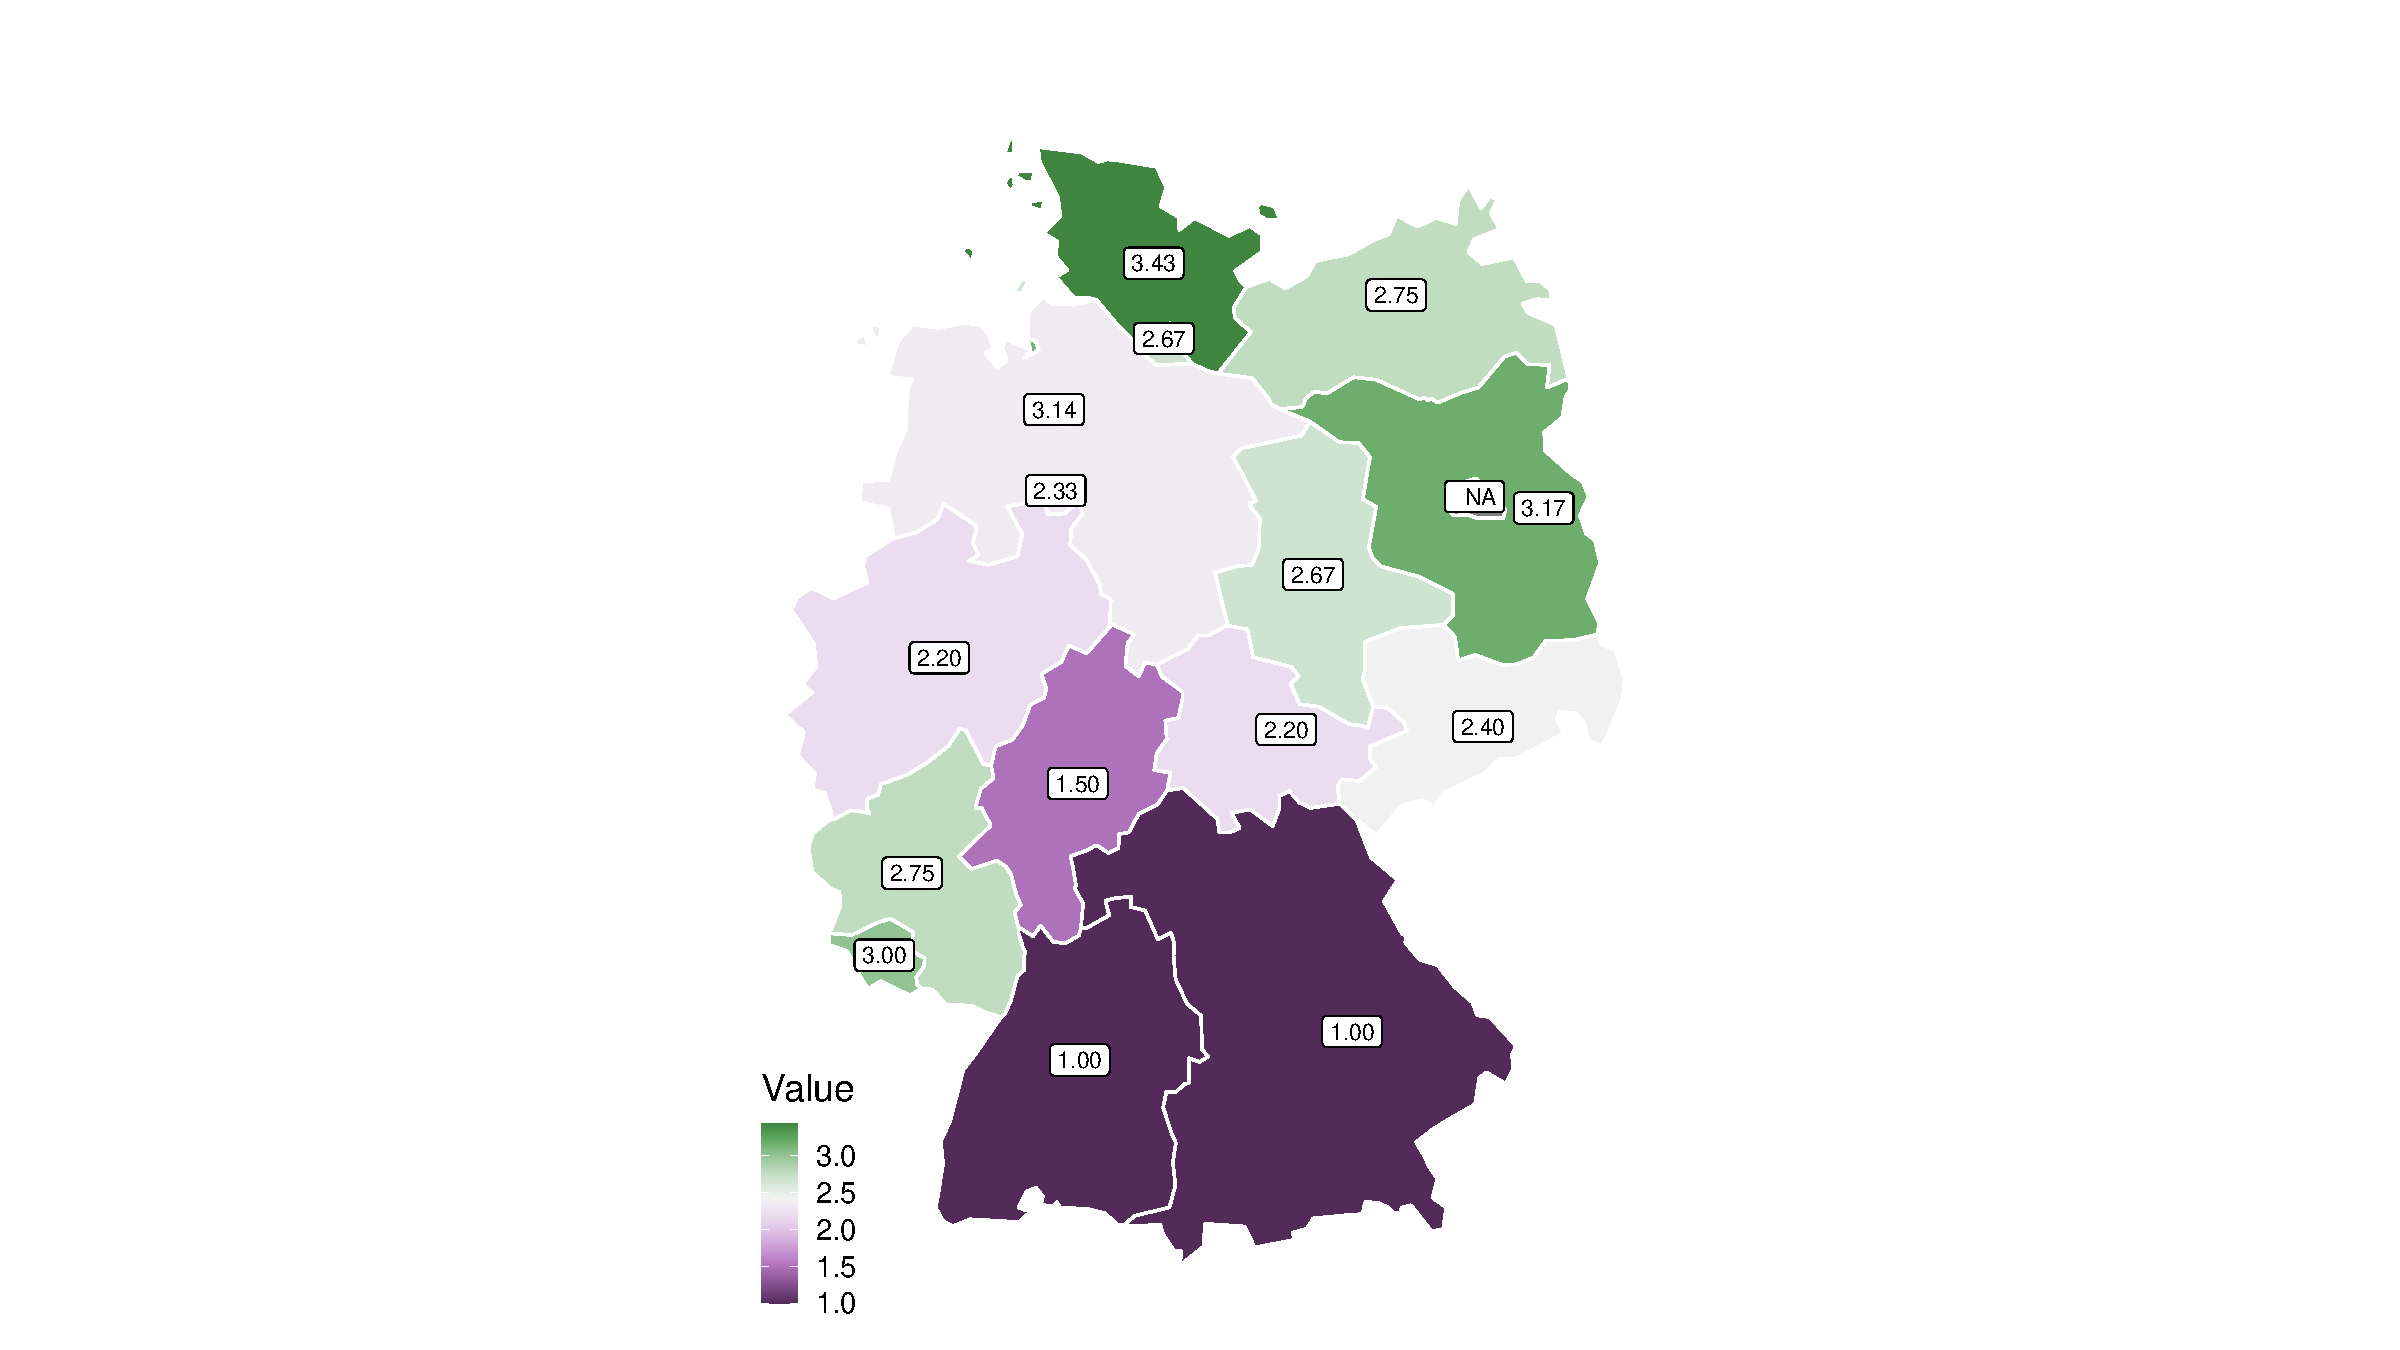
\includegraphics[width = \linewidth]{fedattAVG.pdf}
	\caption{States' attitudes toward federalism (average values). Source: \citep{BarbaroRode2024}}
	%	\newline Attitudes toward federalism are measured on a scale of 1 (strongly federalistic, prefers decentralization) to 4 (strongly favors centralized decision-making)
	\label{fig.attitudemap}
\end{figure}

\newpage
\section{Regression Results with detailed covariates} \label{app.fullregtab}
\begin{table}[htbp] 
\centering
\caption{Covid-19 incidence rates and state prime ministers' statements favoring (de)centralized decision-making}
 \label{tb.appendixtable}
	\begin{tabular}{lcc} \toprule
		& (1) & (2)  \\ \midrule
ln(state-level incidence rate) & 1.983** & 1.985** \\
	&	[1.30,3.02]  & [1.29,3.06] \\
  & & \\
ln(state-level vacc. rate) & & 0.806 \\
		&  & [0.606,1.072] \\
   & & \\
State's general stance towards federalism & 0.850 & 0.826 \\
\, (1 = decentralization, $\ldots$ 4 = centralization ) & [0.566,1.270] & [0.548,1.24] \\
 & & \\
State's financial strength (mean 94, SD 17) & 0.990 & 0.989 \\
        & [0.968,1.01] & [0.967,1.01] \\
         & & \\
State's share of the manufacturing sector  & 0.161 & 0.136 \\
\, in gross value added        & [0.004,6.710] & [0.003,5.752]  \\ 
		& &  \\
Linear time trend & Yes & Yes \\
		& &  \\
Dummies for Eastern  &    &     \\
\,  states and Berlin  & Yes & Yes \\ 
		& &  \\ \bottomrule 
	\end{tabular}
\begin{minipage}{\textwidth}
\small
\textit{Notes:} 
This table corresponds to columns (4) and (5) in Table \ref{tb.mainreg}, with the difference that the state-level controls are reported individually. For explanations of the values, we refer to the description of Table \ref{tb.mainreg}.
 %Each column reports exponentiated coefficients from a separate ordered logit regression. Dependent variable is the 4-point pandemic policy index (PPI). Higher values indicate a stronger expressed desire for centralized decision-making. Coefficients are expressed as changes in the odds ratio of giving a statement $Y$ that falls into a higher vs a lower category $j$, i.e., $P(Y\leq j)/P(Y > j)$. All regressions control for ln(federal level incidence rate) and column (5) additionally controls for ln(federal level vaccination rate) and a dummy for the pre-vaccination period. State-level controls include states' general stances towards federalism, share of the manufacturing sector in gross value added, and financial strength ("Finanzkraftmesszahl"). 
 \newline \textit{*** $p < 0.01$, ** $p < 0.05$, * $p < 0.10$}
	\end{minipage}
\end{table}

%\newpage  

\bibliographystyle{elsarticle-harv} 
\bibliography{ber}




\subsection*{Funding, Conflict of interest}
The authors declare: no funding received for conducting this work, no conflict of interests.


\end{document}

\endinput
%%
%% End of file `elsarticle-template-harv.tex'.

